%%%%%%%%%%%%%%%%%%%%%%%%%%%%%%%%%%%%%%%%%%%%%%%%%%%
%
%  New template code for TAMU Theses and Dissertations starting Fall 2012.  
%  For more info about this template or the 
%  TAMU LaTeX User's Group, see http://www.howdy.me/.
%
%  Author: Wendy Lynn Turner 
%	 Version 1.0 
%  Last updated 8/5/2012
%
%%%%%%%%%%%%%%%%%%%%%%%%%%%%%%%%%%%%%%%%%%%%%%%%%%%
%%%                           APPENDIX - Chapter 3
%%%%%%%%%%%%%%%%%%%%%%%%%%%%%%%%%%%%%%%%%%%%%%%%%%%

\phantomsection
\chapter{\uppercase{Addendum to Chapter \ref{sec::BF}}}
\label{sec::appendix_BF}

%%%%%%%%%%%%%%%%%%%%%%%%%%%%%%%%%%%%%%%%%%%%%%%%%%%
%%%   Section - Limits of the Linear Polygonal Basis Functions
\section{Limits of the Linear Polygonal Basis Functions}
\label{sec::appendix_BF_Limits}

As it was stated in Chapter \ref{sec::B}, the Wachspress, mean value, and maximum entropy coordinates are all undefined on the boundary of the polygonal element. However, these basis functions do have a valid limit on the boundary. This means that while direct boundary evaluation of the coordinates is impossible (results in divide-by-zero issues), we can demonstrate that the limits of their values are exactly those required of general barycentric coordinates. We use the geometric properties for an arbitrary polygon presented in Figure \ref{fig::App_BF_2D_ref_polygon} to do this.

\begin{figure}
\centering
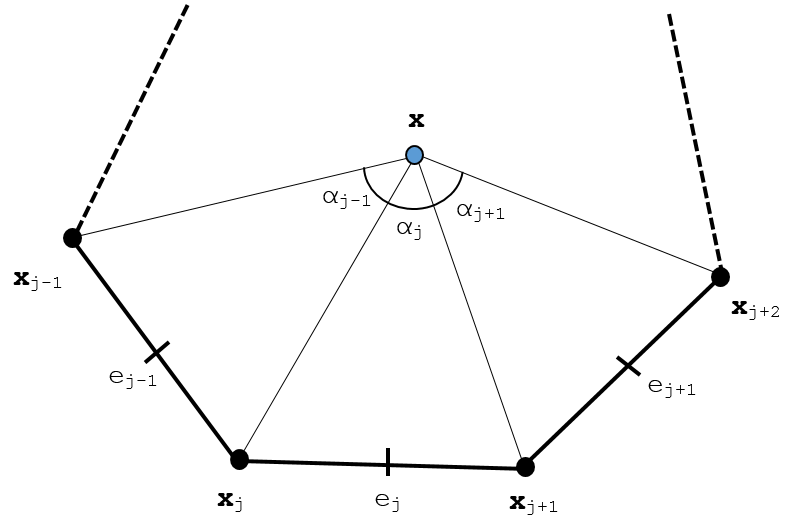
\includegraphics[width=0.65\textwidth]{figures/appendices/ref_polygon.png}
\caption{Arbitrary polygon with geometric properties used for 2D basis function generation.}
\label{fig::App_BF_2D_ref_polygon}
\end{figure}

%%%%%%%%%%%%%%%%%%%%%%%%%%%%%%%%%%%%%%%%%%%%%%%%%%%
%%%  Sub Section - Wachspress Limits
\subsection{Limits of the Wachspress Coordinates}
\label{sec::appendix_BF_Limits_Wachspress}

Recall from Section \ref{sec::BF_2DLinear_Wachspress} that the Wachspress basis functions on a polygon $K$ with $N_K$ vertices are of the form

\begin{equation}
\label{eq::App_BF_WachBF}
\lambda_i (\vec{x}) = \frac{w_i  (\vec{x}) }{\sum\limits_{j=1}^{N_K} w_j  (\vec{x}) },
\end{equation}

\noindent where the weight function for vertex $i$, $w_i$, has the following definition:

\begin{equation}
\label{eq::App_BF_wach_weights}
w_i (\vec{x})  = \frac{A(\vec{x}_{i-1}, \vec{x}_{i}, \vec{x}_{i+1})}{A(\vec{x}, \vec{x}_{i-1}, \vec{x}_{i}) \, A(\vec{x}, \vec{x}_{i}, \vec{x}_{i+1})} .
\end{equation}

First, we analyze the limiting case as the point of evaluation, $\vec{x}$, approaches a vertex. The Wachspress coordinates maintain the {\em Lagrange property}: $\lambda_i (\vec{x}_j)=\delta_{ij}$. We prove this now by first dividing the numerator and denominator of Eq. (\ref{eq::App_BF_WachBF}) through by $w_j$ to yield the following:

\begin{equation}
\label{eq::App_BF_wach_divide}
\lambda_i (\vec{x}) = \frac{w_i/w_j}{1+\sum\limits_{k\neq j} w_k/w_j}, \, i \neq j \qquad \text{and} \qquad \lambda_j (\vec{x}) = \frac{1}{1+\sum\limits_{k\neq j} w_k/w_j} .
\end{equation}

\noindent Next, we define the term $R_{i,j}$ to be the following

\begin{equation}
\label{eq::App_BF_wach_R}
R_{i,j}(\vec{x}) = \frac{w_i (\vec{x})}{w_j (\vec{x})} .
\end{equation}

\noindent Using the definition of Eq. (\ref{eq::App_BF_wach_R}), we can rewrite Eq. (\ref{eq::App_BF_wach_divide}) as the following 

\begin{equation}
\label{eq::App_BF_wach_divideR}
\lambda_i (\vec{x}) = \frac{R_{i,j}}{1+\sum\limits_{k\neq j} R_{k,j}}, \, i \neq j \qquad \text{and} \qquad \lambda_j (\vec{x}) = \frac{1}{1+\sum\limits_{k\neq j} R_{k,j}} .
\end{equation}

\noindent It is obvious from Eq. (\ref{eq::App_BF_wach_divideR}) that if all the $R_{k,j}$ ($k \neq j$) and $R_{i,j}$ ($i \neq j$) terms are zero, then we capture the {\em Lagrange property} for the mean value coordinates. Therefore, we expand the terms of $R_{i,j}$ to give Eq. (\ref{eq::App_BF_wach_R_expand}).

\begin{equation}
\label{eq::App_BF_wach_R_expand}
R_{i,j}(\vec{x}) = \frac{A(\vec{x}_{i-1}, \vec{x}_{i}, \vec{x}_{i+1})}{A(\vec{x}_{j-1}, \vec{x}_{j}, \vec{x}_{j+1})} \, \frac{A(\vec{x}_{j-1}, \vec{x}_{j}, \vec{x}) A(\vec{x}_{j}, \vec{x}_{j+1}, \vec{x})}{A(\vec{x}_{i-1}, \vec{x}_{i}, \vec{x}) A(\vec{x}_{i}, \vec{x}_{i+1}, \vec{x})}
\end{equation}

\noindent From Eq. (\ref{eq::App_BF_wach_R_expand}), it is clear that the first term is bounded and non-zero and that the following limit is true:

\begin{equation}
\label{eq::App_BF_wach_vertlim}
\lim\displaylimits_{\vec{x}\rightarrow \vec{x}_j} \left(  \frac{A(\vec{x}_{j-1}, \vec{x}_{j}, \vec{x}) A(\vec{x}_{j}, \vec{x}_{j+1}, \vec{x})}{A(\vec{x}_{i-1}, \vec{x}_{i}, \vec{x}) A(\vec{x}_{i}, \vec{x}_{i+1}, \vec{x})} \right) = 0
\end{equation}

\noindent Therefore, the following is true,

\begin{equation}
\label{eq::App_BF_wach_Rlim}
\lim\displaylimits_{\vec{x} \rightarrow \vec{x}_j} R_{i,j}(\vec{x}) = 0 ,
\end{equation} 

\noindent and the {\em Lagrange property} holds for the Wachspress coordinates:

\begin{equation}
\label{eq::App_BF_wach_vertFINAL}
\lambda_i (\vec{x}) = \delta_{ij}.
\end{equation} 

Next, we seek to show that the Wachspress coordinates have piecewise linearity on the boundary of the polygon $K$. Therefore, we will analyze the limit of the basis functions as the point $\vec{x}$ approaches face $e_j$. This limit is formally defined as the following

\begin{equation}
\label{eq::App_BF_wach_edge_lim_init}
\lim\displaylimits_{\vec{x} \rightarrow \vec{x}^* \in e_j}  \lambda_i (\vec{x}) .
\end{equation} 

\noindent From the definitions of the vertex weight functions of Eq. (\ref{eq::App_BF_wach_weights}), we can immediately see that 

\begin{equation}
\label{eq::App_BF_wach_edge_lim_jj1}
\lim\displaylimits_{\vec{x} \rightarrow \vec{x}^* \in e_j} | w_i (\vec{x}) |= \infty, \qquad i=(j,j+1) ,
\end{equation} 

\noindent and

\begin{equation}
\label{eq::App_BF_wach_edge_lim_others}
\lim\displaylimits_{\vec{x} \rightarrow \vec{x}^* \in e_j} |  w_i (\vec{x}) | < \infty, \qquad i\neq (j,j+1) .
\end{equation} 

\noindent Therefore, the following is also true for the basis functions

\begin{equation}
\label{eq::App_BF_wach_edge_lim_bfj}
\lim\displaylimits_{\vec{x} \rightarrow \vec{x}^* \in e_j}  \lambda_i (\vec{x}) = 0, \qquad i\neq(j,j+1),
\end{equation} 

\noindent and

\begin{equation}
\label{eq::App_BF_wach_edge_lim_bfj}
\lim\displaylimits_{\vec{x} \rightarrow \vec{x}^* \in e_j}  \lambda_{j} (\vec{x}) = \frac{w_j}{w_j + w_{j+1}}, 
\end{equation} 

\noindent and

\begin{equation}
\label{eq::App_BF_wach_edge_lim_bfj1}
\lim\displaylimits_{\vec{x} \rightarrow \vec{x}^* \in e_j}  \lambda_{j+1} (\vec{x}) = \frac{w_{j+1}}{w_j + w_{j+1}}.
\end{equation} 

\noindent We expand the term $\lambda_j$ as the following,

\begin{equation}
\label{eq::App_BF_wach_edge_lim_lamj_expand}
\lim\displaylimits_{\vec{x} \rightarrow \vec{x}^* \in e_j}  \lambda_{j} (\vec{x}) = \frac{A(\vec{x}_{j-1}, \vec{x}_{j}, \vec{x}_{j+1}) \, A(\vec{x}_{j+1}, \vec{x}_{j+2}, \vec{x})}{A(\vec{x}_{j-1}, \vec{x}_{j}, \vec{x}_{j+1}) \, A(\vec{x}_{j+1}, \vec{x}_{j+2}, \vec{x}) + A(\vec{x}_{j}, \vec{x}_{j+1}, \vec{x}_{j+2}) \, A(\vec{x}_{j-1}, \vec{x}_{j}, \vec{x})},
\end{equation} 

\noindent or

\begin{equation}
\label{eq::App_BF_wach_edge_lim_lamj_expand2}
\lim\displaylimits_{\vec{x} \rightarrow \vec{x}^* \in e_j}  \lambda_{j} (\vec{x}) = \frac{1}{1+\beta},
\end{equation} 

\noindent where

\begin{equation}
\label{eq::App_BF_wach_beta}
\beta = \frac{A(\vec{x}_{j}, \vec{x}_{j+1}, \vec{x}_{j+2}) \, A(\vec{x}_{j-1}, \vec{x}_{j}, \vec{x})}{A(\vec{x}_{j-1}, \vec{x}_{j}, \vec{x}_{j+1}) \, A(\vec{x}_{j+1}, \vec{x}_{j+2}, \vec{x}) }. 
\end{equation} 

\noindent Through extensive algebra along with the use of some trigonometric properties and further limits, the $\beta$ term can be written as the following 

\begin{equation}
\label{eq::App_BF_wach_beta2}
\beta = \frac{|\vec{x}_{j} - \vec{x}|}{|\vec{x}_{j+1} - \vec{x}|}, 
\end{equation} 

\noindent which means that the limit of $\lambda_{j}$ can be written as the following as well:

\begin{equation}
\label{eq::App_BF_wach_edge_lim_lamj_expand3}
\lim\displaylimits_{\vec{x} \rightarrow \vec{x}^* \in e_j}  \lambda_{j} (\vec{x}) = \frac{|\vec{x}_{j+1} - \vec{x}|}{|\vec{x}_{j+1} - \vec{x}_j|} .
\end{equation} 

\noindent Through a similar procedure, the limit of $\lambda_{j+1}$ can be written as the following as well:

\begin{equation}
\label{eq::App_BF_wach_edge_lim_lamj1_expand3}
\lim\displaylimits_{\vec{x} \rightarrow \vec{x}^* \in e_j}  \lambda_{j+1} (\vec{x}) = \frac{|\vec{x}_{j} - \vec{x}|}{|\vec{x}_{j+1} - \vec{x}_j|} .
\end{equation} 

\noindent respectively. Therefore, we can write the final result for the boundary analysis of the Wachspress coordinates in Eq. (\ref{eq::App_BF_wach_faceFINAL}).

\begin{equation}
\label{eq::App_BF_wach_faceFINAL}
\lim\displaylimits_{\vec{x} \rightarrow \vec{x}^* \in e_j} \lambda_i (\vec{x}) = 
\begin{cases}
\frac{| \vec{x}_{j+1} - \vec{x} |}{| \vec{x}_{j+1} - \vec{x}_{j} |},&i=j\\
\frac{| \vec{x}_{j} - \vec{x} |}{| \vec{x}_{j+1} - \vec{x}_{j} |},&i=j+1\\
\,0,&\text{otherwise}
\end{cases}
\end{equation} 

%%%%%%%%%%%%%%%%%%%%%%%%%%%%%%%%%%%%%%%%%%%%%%%%%%%
%%%  Sub Section - MV Limits
\subsection{Limits of the Mean Value Coordinates}
\label{sec::appendix_BF_Limits_MV}

Recall from Section \ref{sec::BF_2DLinear_MV} that the mean value basis functions on a polygon $K$ with $N_K$ vertices are of the form

\begin{equation}
\label{eq::App_BF_MVBF}
\lambda_i (\vec{x}) = \frac{w_i  (\vec{x}) }{\sum\limits_{j=1}^{N_K} w_j  (\vec{x}) }
\end{equation}

\noindent where the weight function for vertex $i$, $w_i$, has the following definition:

\begin{equation}
\label{eq::App_BF_MV_weights}
w_i (\vec{x})  = \frac{\tan(\alpha_{i-1} / 2) + \tan(\alpha_i / 2)}{|\vec{x}_i - \vec{x}|}
\end{equation}

First, we analyze the limiting case as the point of evaluation, $\vec{x}$, approaches the vertex $j$, $\vec{x}_j$. The mean value coordinates maintain the {\em Lagrange property}: $\lambda_i (\vec{x}_j)=\delta_{ij}$. We prove this now by first dividing the numerator and denominator of Eq. (\ref{eq::App_BF_MVBF}) through by $w_j$ to yield the following:

\begin{equation}
\label{eq::App_BF_MV_divide}
\lambda_i (\vec{x}) = \frac{w_i/w_j}{1+\sum\limits_{k\neq j} w_k/w_j}, \, i \neq j \qquad \text{and} \qquad \lambda_j (\vec{x}) = \frac{1}{1+\sum\limits_{k\neq j} w_k/w_j} .
\end{equation}

\noindent Next, we define the term $R_{i,j}$ to be the following

\begin{equation}
\label{eq::App_BF_MV_R}
R_{i,j}(\vec{x}) = \frac{w_i (\vec{x})}{w_j (\vec{x})} .
\end{equation}

\noindent Using the definition of Eq. (\ref{eq::App_BF_MV_R}), we can rewrite Eq. (\ref{eq::App_BF_MV_divide}) as the following 

\begin{equation}
\label{eq::App_BF_MV_divideR}
\lambda_i (\vec{x}) = \frac{R_{i,j}}{1+\sum\limits_{k\neq j} R_{k,j}}, \, i \neq j \qquad \text{and} \qquad \lambda_j (\vec{x}) = \frac{1}{1+\sum\limits_{k\neq j} R_{k,j}} .
\end{equation}

\noindent It is obvious from Eq. (\ref{eq::App_BF_MV_divideR}) that if all the $R_{k,j}$ ($k \neq j$) and $R_{i,j}$ ($i \neq j$) terms are zero, then we capture the {\em Lagrange property} for the mean value coordinates. Therefore, we expand the terms of $R_{i,j}$ to give Eq. (\ref{eq::App_BF_MV_R_expand}).

\begin{equation}
\label{eq::App_BF_MV_R_expand}
\begin{aligned}
R_{i,j}(\vec{x}) = \frac{w_i}{w_j}  &= \frac{\tan (\alpha_{i-1}/2) + \tan (\alpha_{i}/2)}{| \vec{x}_i - \vec{x} |} \frac{| \vec{x}_j - \vec{x} |}{\tan (\alpha_{j-1}/2) + \tan (\alpha_{j}/2)} \\ \\
&= \frac{| \vec{x}_j - \vec{x} |}{| \vec{x}_i - \vec{x}|} \frac{\tan (\alpha_{i-1}/2) + \tan (\alpha_{i}/2)}{\tan (\alpha_{j-1}/2) + \tan (\alpha_{j}/2)}
\end{aligned}
\end{equation}

\noindent Next, we define the following trigonometric property:

\begin{equation}
\label{eq::App_BF_MV_trig}
\tan(x) + \tan(y) = \frac{\sin(x+y)}{\cos(x) \cos(y)} .
\end{equation} 

\noindent Inserting Eq. (\ref{eq::App_BF_MV_trig}) into the final line of Eq. (\ref{eq::App_BF_MV_R_expand}), we obtain:

\begin{equation}
\label{eq::App_BF_MV_R_wtrig}
R_{i,j}(\vec{x}) = \frac{| \vec{x}_j - \vec{x} |}{| \vec{x}_i - \vec{x} |} \frac{\sin (\alpha_{i-1}/2 + \alpha_{i}/2)}{\sin (\alpha_{j-1}/2 + \alpha_{j}/2)} \frac{\cos (\alpha_{j-1}/2) \cos (\alpha_{j}/2)}{\cos (\alpha_{i-1}/2) \cos (\alpha_{i}/2)} .
\end{equation} 

\noindent In the limit as $\vec{x}$ approaches $\vec{x}_j$, we see that the term $|| \vec{x}_j - \vec{x} ||$ approaches zero. However, we need to assess what the other terms in Eq. (\ref{eq::App_BF_MV_R_wtrig}) will approach. If we examine the limiting cases where $\vec{x}_i = \vec{x}_{j-1}$ or $\vec{x}_i = \vec{x}_{j}$, then the limits of the remaining terms of Eq. (\ref{eq::App_BF_MV_R_wtrig}) can be written as the following.

\begin{equation}
\label{eq::App_BF_MV_R_terms}
\begin{aligned}
\lim\displaylimits_{\vec{x} \rightarrow \vec{x}_j}  | \vec{x}_i - \vec{x} |  > 0 \\
\lim\displaylimits_{\vec{x} \rightarrow \vec{x}_j} \left|  \sin (\alpha_{i-1}/2 + \alpha_{i}/2) \right| > 0 \\
\lim\displaylimits_{\vec{x} \rightarrow \vec{x}_j} \left|  \sin (\alpha_{j-1}/2 + \alpha_{j}/2) \right| > 0 \\
\lim\displaylimits_{\vec{x} \rightarrow \vec{x}_j} \left|  \cos (\alpha_{i-1}/2) \right| > 0 \\
\lim\displaylimits_{\vec{x} \rightarrow \vec{x}_j} \left|  \cos (\alpha_{i}/2) \right| > 0 \\
\lim\displaylimits_{\vec{x} \rightarrow \vec{x}_j} \left|  \cos (\alpha_{j-1}/2) \right| > 0 \\
\lim\displaylimits_{\vec{x} \rightarrow \vec{x}_j} \left|  \cos (\alpha_{j}/2) \right| > 0
\end{aligned}
\end{equation}

\noindent Therefore, the following is true,

\begin{equation}
\label{eq::App_BF_MV_Rlim}
\lim\displaylimits_{\vec{x} \rightarrow \vec{x}_j} R_{i,j}(\vec{x}) = 0 ,
\end{equation} 

\noindent and the {\em Lagrange property} holds for the mean value coordinates:

\begin{equation}
\label{eq::App_BF_MV_vertFINAL}
\lambda_i (\vec{x}) = \delta_{ij}.
\end{equation} 

Next, we seek to show that the mean value coordinates have piecewise linearity on the boundary of the polygon $K$. Therefore, we will analyze the limit of the basis functions as the point $\vec{x}$ approaches face $e_j$. This limit is formally defined as the following

\begin{equation}
\label{eq::App_BF_MV_edge_lim_init}
\lim\displaylimits_{\vec{x} \rightarrow \vec{x}^* \in e_j}  \lambda_i (\vec{x}) .
\end{equation} 

\noindent If we define the signed area function, $A_j (\vec{x})$, for face, $e_j$,


\begin{equation}
\label{eq::App_BF_MV_weights_mod}
A_j (\vec{x}) = \frac{1}{2} 
\left|
\begin{array}{ccc}
1&1&1\\
x&x_j&x_{j+1}\\
y&y_j&y_{j+1}
\end{array}
\right|
= \frac{| \vec{x}_j - \vec{x} | \,| \vec{x}_{j+1} - \vec{x} | \sin (\alpha_j)}{2}
\end{equation}

\noindent then a modified vertex weight function, $\hat{w}_i$, can be given as

\begin{equation}
\label{eq::App_BF_MV_weights_mod}
\hat{w}_i (\vec{x})  = w_i (\vec{x}) A_j (\vec{x}) .
\end{equation}

\noindent This modified weight functions can be expanded to

\begin{equation}
\label{eq::App_BF_MV_weights_mod_expand}
\hat{w}_i (\vec{x})  = \frac{\tan(\alpha_{i-1} / 2) + \tan(\alpha_i / 2)}{|\vec{x}_i - \vec{x}|} \frac{| \vec{x}_j - \vec{x} | \,|\vec{x}_{j+1} - \vec{x} | \sin (\alpha_j)}{2},
\end{equation}

\noindent and the mean value basis functions can be rewritten in terms of these modified functions:

\begin{equation}
\label{eq::App_BF_MVBF_mod}
\lambda_i (\vec{x}) = \frac{\hat{w}_i  (\vec{x}) }{\sum\limits_{j=1}^{N_K} \hat{w}_j  (\vec{x}) }
\end{equation}

\noindent Analyzing Eq. (\ref{eq::App_BF_MV_weights_mod_expand}), we can immediately discern that $\hat{w}_i (\vec{x}) = 0 $ for ($i=j,j+1$). This is because as $\vec{x}$ goes to the boundary, $\alpha_j$ goes to $\pi$ and $\sin (\alpha_j)$ goes to zero. We will show below that the limit of $\hat{w}_i (\vec{x}) $ is greater than zero and bounded for ($i=j,j+1$). We can then write the mean value basis functions in the modified terms for vertex $j$ and $j+1$ as 

\begin{equation}
\label{eq::App_BF_MVBF_mod_j}
\lambda_j (\vec{x}) = \frac{\hat{w}_j  }{\hat{w}_j+ \hat{w}_{j+1} } ,
\end{equation}

\noindent and

\begin{equation}
\label{eq::App_BF_MVBF_mod_j1}
\lambda_{j+1} (\vec{x}) = \frac{\hat{w}_{j+1}   }{\hat{w}_j+ \hat{w}_{j+1} } ,
\end{equation}

\noindent respectively. Taking the limits of the modified weight functions for vertex $j$ and $j+1$ gives

\begin{equation}
\label{eq::App_BF_MVBF_weightmod_j}
\lim\displaylimits_{\vec{x} \rightarrow \vec{x}^* \in e_j}\hat{w}_j (\vec{x}) =  | \vec{x}_{j+1} - \vec{x} |,
\end{equation}

\noindent and

\begin{equation}
\label{eq::App_BF_MVBF_weightmod_j1}
\lim\displaylimits_{\vec{x} \rightarrow \vec{x}^* \in e_j} \hat{w}_{j+1} (\vec{x}) = | \vec{x}_j - \vec{x} |,
\end{equation}

\noindent respectively. Therefore, we can write the final result for the boundary analysis of the mean value coordinates in Eq. (\ref{eq::App_BF_MV_faceFINAL}).

\begin{equation}
\label{eq::App_BF_MV_faceFINAL}
\lim\displaylimits_{\vec{x} \rightarrow \vec{x}^* \in e_j} \lambda_i (\vec{x}) = 
\begin{cases}
\frac{| \vec{x}_{j+1} - \vec{x} |}{| \vec{x}_{j+1} - \vec{x}_{j} |},&i=j\\
\frac{| \vec{x}_{j} - \vec{x} |}{| \vec{x}_{j+1} - \vec{x}_{j} |},&i=j+1\\
\,0,&\text{otherwise}
\end{cases}
\end{equation} 

%%%%%%%%%%%%%%%%%%%%%%%%%%%%%%%%%%%%%%%%%%%%%%%%%%%
%%%  Sub Section - ME Limits
\subsection{Limits of the Maximum Entropy Coordinates}
\label{sec::appendix_BF_Limits_ME}

Recall from Section \ref{sec::BF_2DLinear_ME} that the maximum entropy basis functions on a polygon $K$ with $N_K$ vertices are of the form

\begin{equation}
\label{eq::App_BF_MEBF}
\lambda_i (\vec{x}) = \frac{w_i  (\vec{x}) }{\sum\limits_{j=1}^{N_K} w_j  (\vec{x}) }
\end{equation}

\noindent where the weight function for vertex $i$, $w_i$, has the following definition

\begin{equation}
\label{eq::App_BF_ME_weights}
w_i (\vec{x})  = m_i(\vec{x}) \exp(-  \vec{\kappa} \cdot (\vec{x}_i - \vec{x})).
\end{equation}

\noindent In Eq. (\ref{eq::App_BF_ME_weights}), the prior distribution, $m_i$, has the form 

\begin{equation}
\label{eq::BF_ME_prior_funcs}
 m_i(\vec{x}) = \frac{\pi_i (\vec{x}) }{\sum\limits_{k=1}^{N_K} \pi_k (\vec{x})},
\end{equation}

\noindent where

\begin{equation}
\label{eq::BF_ME_prior_products}
\pi_i (\vec{x}) = \prod\limits_{k \neq i-1, i}^{N_K} \rho_k (\vec{x}),
\end{equation}

\noindent and

\begin{equation}
\label{eq::BF_ME_face_funcs}
\rho_j (\vec{x}) = || \vec{x} - \vec{x}_j || + || \vec{x} - \vec{x}_{j+1} || - || \vec{x}_{j+1} - \vec{x}_j || ,
\end{equation}

\noindent and $\rho_j$ is the face weight function corresponding to face $e_j$. The weight function for face $e_j$ is identically zero along face $e_j$ and strictly positive elsewhere by the Triangle Inequality. This means that the product $\pi_i$ and the prior distribution $ m_i$ for vertex $i$ is zero on all faces that do not touch vertex $i$.

We do not have an exact proof that 

For the maximum entropy coordinates, we will only demonstrate the piecewise linearity property since the {\em Lagrange property} is satisfied by the limit at the face vertices.

%%%%%%%%%%%%%%%%%%%%%%%%%%%%%%%%%%%%%%%%%%%%%%%%%%%
%%%   Section - Jacobian
\section{Jacobian Transformations of the Reference Element}
\label{sec::appendix_BF_Jac}

In Section \ref{sec::BF_2DIntegration}, we provided the details for numerically integrating the elementary matrices on arbitrary polygons. This was done by triangulation of the polygon $K$ with $N_K$ into $N_K$ distinct sub-triangles. Quadrature nodes and weights were selected on the reference triangle with vertices $\left[  (0,0),(1,0),(0,1) \right]$. Then, this reference quadrature set was affinely mapped onto the different sub-triangles of $K$. This mapping of points from the reference space into the global space was performed with a Jacobian transformation. The visual depiction for this mapping is given in Figure \ref{fig::App_BF_2D_tri_mapping}. We now provide greater details of this Jacobian transformation.

\begin{figure}
\centering
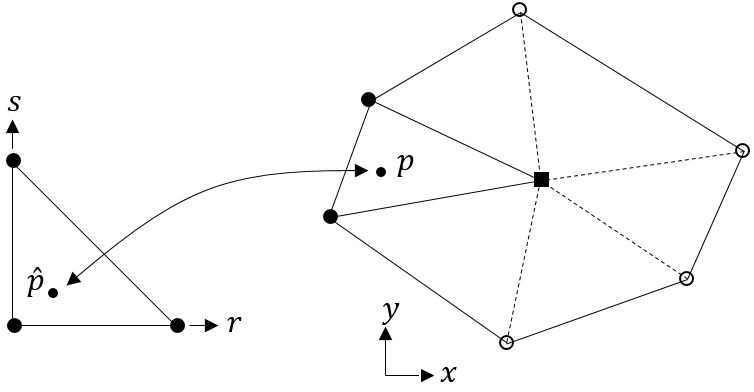
\includegraphics[width=0.75\textwidth]{figures/appendices/triangle_mapping_Rev1.png}
\caption{Mapping a point on the reference triangle onto a sub-triangle of an arbitrary polygon.}
\label{fig::App_BF_2D_tri_mapping}
\end{figure}



%%%%%%%%%%%%%%%%%%%%%%%%%%%%%%%%%%%%%%%%%%%%%%%%%%%
%%%   Section - Analytical 2D PWL Integration
\section{Analytical Integration of the PWL Basis Functions}
\label{sec::appendix_BF_PWLInt}

In Chapter \ref{sec::BF}, we provided the functional form for the Piecewise Linear (PWL) coordinates in 2D and 3D. At that time, we simply left the notation for the basis functions and did not give any further information except that a quadrature scheme could be used to integrate the elementary matrices. However, since the PWL coordinates are collections of polynomials over sub-triangles and sub-tetrahedra in 2D and 3D, respectively, direct analytical integration can also be performed. In this section, we detail how the elementary matrices can be integrated with the PWL functions.

%%%%%%%%%%%%%%%%%%%%%%%%%%%%%%%%%%%%%%%%%%%%%%%%%%%
%%%  Sub Section - 2D integration
\subsection{2D PWL Basis Functions}
\label{sec::appendix_BF_PWLInt_2D}

In Section \ref{sec::BF_2DLinear_PWL}, we provided the functional form for the 2D Piecewise Linear (PWL) coordinates. We noted that of the linearly-complete 2D polygonal coordinates, PWL is the only one that can perform analytical integrations of the elementary matrices. We now describe the procedures to perform these analytical integrations of the elementary matrices.

\begin{equation}
\label{eq::App_BF_2D_triref_massterm}
\begin{aligned}
\int\displaylimits_K b_i b_j &= \int\displaylimits_K \left( t_i + \alpha_K t_c  \right) \left(  t_j + \alpha_K t_c \right) \\
&= \int\displaylimits_K t_i t_j + \alpha_K \int\displaylimits_K t_i t_c + \alpha_K \int\displaylimits_K t_j t_c + \alpha_K^2 \int\displaylimits_K t_c t_c
\end{aligned}
\end{equation}

\begin{equation}
\label{eq::App_BF_2D_triref_gradterm}
\begin{aligned}
\int\displaylimits_K \vec{\nabla} b_i \,  b_j &= \int\displaylimits_K \left( \vec{\nabla} t_i + \alpha_K \vec{\nabla} t_c  \right) \left(  t_j + \alpha_K t_c \right) \\
&= \int\displaylimits_K \vec{\nabla} t_i \,t_j + \alpha_K \int\displaylimits_K \vec{\nabla} t_i\, t_c + \alpha_K \int\displaylimits_K t_j \vec{\nabla} t_c + \alpha_K^2 \int\displaylimits_K \vec{\nabla} t_c \, t_c
\end{aligned}
\end{equation}


\begin{equation}
\label{eq::App_BF_2D_triref}
\begin{aligned}
	\hat{b}_1(r,s) & = 1-r-s \\
	\hat{b}_2(r,s) & = r \\
	\hat{b}_3(r,s) & = s 
\end{aligned}
\end{equation}

\begin{equation}
\label{eq::App_BF_2D_triref_grad}
\vec{\nabla} \hat{b} (r,s)  = 
\left[
\begin{array}{cc}
-1 & -1 \\
1 & 0 \\
0 & 1
\end{array}
\right]
\end{equation}

%%%%%%%%%%%%%%%%%%%%%%%%%%%%%%%%%%%%%%%%%%%%%%%%%%%
%%%  Sub Section - 3D integration
\subsection{3D PWL Basis Functions}
\label{sec::appendix_BF_PWLInt_3D}



\begin{equation}
\label{eq::3D_tetref_BF}
\begin{aligned}
	\hat{b}_1(r,s,t) & = 1-r-s-t \\
	\hat{b}_2(r,s,t) & = r \\
	\hat{b}_3(r,s,t) & = s \\
	\hat{b}_4(r,s,t) & = t
\end{aligned}
\end{equation}

\begin{equation}
\label{eq::App_BF_3D_tetref_grad}
\vec{\nabla} \hat{b} (r,s,t)  = 
\left[
\begin{array}{ccc}
-1 & -1 & -1 \\
1 & 0 & 0 \\
0 & 1 & 0 \\
0 & 0 & 1
\end{array}
\right]
\end{equation}
